% Made up for the tikra benchmark.
\usetikzlibrary{matrix}
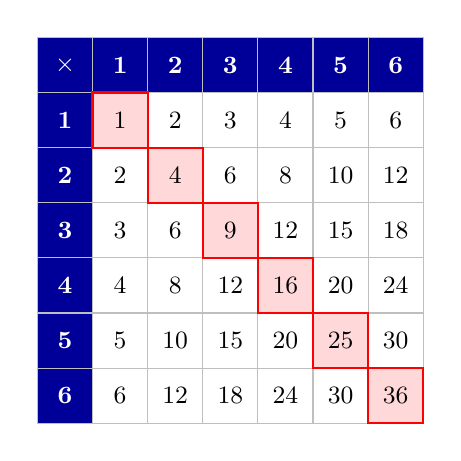
\begin{tikzpicture}
  \matrix (m) [matrix of nodes, nodes={draw=gray!50, minimum size=7mm, font=\small, anchor=center},
      column sep=-\pgflinewidth, row sep=-\pgflinewidth,
      row 1/.style={nodes={fill=blue!60!black, text=white, font=\small\bfseries}},
      column 1/.style={nodes={fill=blue!60!black, text=white, font=\small\bfseries}}] {
    $\times$ & 1 & 2 & 3 & 4 & 5 & 6 \\
    1 & 1 & 2 & 3 & 4 & 5 & 6 \\
    2 & 2 & 4 & 6 & 8 & 10 & 12 \\
    3 & 3 & 6 & 9 & 12 & 15 & 18 \\
    4 & 4 & 8 & 12 & 16 & 20 & 24 \\
    5 & 5 & 10 & 15 & 20 & 25 & 30 \\
    6 & 6 & 12 & 18 & 24 & 30 & 36 \\
  };
  \foreach \i in {2,...,7}
    \node[draw=red, thick, minimum size=7mm, fill=red!15, font=\small] at (m-\i-\i) {\pgfmathparse{int((\i-1)*(\i-1))}\pgfmathresult};
\end{tikzpicture}
